\documentclass{article}
\usepackage{amsfonts, amsthm, amsmath, amssymb, mathtools, ulem, mathrsfs, physics, esint, siunitx, tikz-cd}
\usepackage{pdfpages, fullpage, color, microtype, cancel, textcomp, markdown, hyperref, graphicx}
\usepackage{enumitem}
\usepackage{algorithm}
\usepackage{algpseudocode}
\graphicspath{{./images/}}
\usepackage[english]{babel}
\usepackage[autostyle, english=american]{csquotes}
\MakeOuterQuote{"}
\usepackage{xparse}
\usepackage{tikz}

\usepackage{calligra}
\DeclareMathAlphabet{\mathcalligra}{T1}{calligra}{m}{n}
\DeclareFontShape{T1}{calligra}{m}{n}{<->s*[2.2]callig15}{}
\newcommand{\script}[1]{\ensuremath{\mathcalligra{#1}}}
\newcommand{\scr}{\script r}

% fonts
\def\mbb#1{\mathbb{#1}}
\def\mfk#1{\mathfrak{#1}}
\def\mbf#1{\mathbf{#1}}
\def\tbf#1{\textbf{#1}}

% common bold letters
\def\bP{\mbb{P}}
\def\bC{\mbb{C}}
\def\bH{\mbb{H}}
\def\bI{\mbb{I}}
\def\bR{\mbb{R}}
\def\bQ{\mbb{Q}}
\def\bZ{\mbb{Z}}
\def\bN{\mbb{N}}

% brackets
\newcommand{\br}[1]{\left(#1\right)}
\newcommand{\sbr}[1]{\left[#1\right]}
\newcommand{\brc}[1]{\left\{#1\right\}}
\newcommand{\lbr}[1]{\left\langle#1\right\rangle}

% vectors
\renewcommand{\i}{\hat{\imath}}
\renewcommand{\j}{\hat{\jmath}}
\renewcommand{\k}{\hat{k}}
\newcommand{\proj}[2]{\text{proj}_{#2}\br{#1}}
\newcommand{\m}[2][b]{\begin{#1matrix}#2\end{#1matrix}}
\newcommand{\arr}[3][\sbr]{#1{\begin{array}{#2}#3\end{array}}}

% misc
\NewDocumentCommand{\seq}{O{n} O{1} O{\infty} m}{\br{#4}_{{#1}={#2}}^{#3}}
\NewDocumentCommand{\app}{O{x} O{\infty}}{\xrightarrow{#1\to#2}}
\newcommand{\sm}{\setminus}
\newcommand{\sse}{\subseteq}
\renewcommand{\ss}{\subset}
\newcommand{\vn}{\varnothing}
\newcommand{\lc}{\epsilon_{ijk}}
\newcommand{\ep}{\epsilon}
\newcommand{\vp}{\varphi}
\renewcommand{\th}{\theta}
\newcommand{\cjg}[1]{\overline{#1}}
\newcommand{\inv}{^{-1}}
\DeclareMathOperator{\im}{im}
\DeclareMathOperator{\id}{id}
\newcommand{\ans}{\tbf{Ans. }}
\newcommand{\pf}{\tbf{Pf. }}
\newcommand{\imp}{\implies}
\newcommand{\impleft}{\reflectbox{$\implies$}}
\newcommand{\ck}{\frac1{4\pi\ep_0}}
\newcommand{\ckb}{4\pi\ep_0}
\newcommand{\sto}{\longrightarrow}
\DeclareMathOperator{\cl}{cl}
\DeclareMathOperator{\intt}{int}
\DeclareMathOperator{\bd}{bd}
\DeclareMathOperator{\Span}{span}
\newcommand{\floor}[1]{\left\lfloor#1\right\rfloor}
\newcommand{\ceil}[1]{\left\lceil#1\right\rceil}
\newcommand{\fxn}[5]{#1:\begin{array}{rcl}#2&\longrightarrow & #3\\[-0.5mm]#4&\longmapsto &#5\end{array}}
\newcommand{\sep}[1][.5cm]{\vspace{#1}}
\DeclareMathOperator{\card}{card}
\renewcommand{\ip}[2]{\lbr{#1,#2}}
\renewcommand{\bar}{\overline}
\DeclareMathOperator{\cis}{cis}
\DeclareMathOperator{\Arg}{Arg}

% title
\title{Scientific Computing HW 6}
\author{Ryan Chen}
%\date{\today}
\setlength{\parindent}{0pt}


\begin{document}
	
\maketitle



\tbf{Problem 1.}

\begin{enumerate}[label=(\alph*)]
	
\item The system $Au=f$ is shown on the left, and the block structure of $A$ is compactly written on the right.

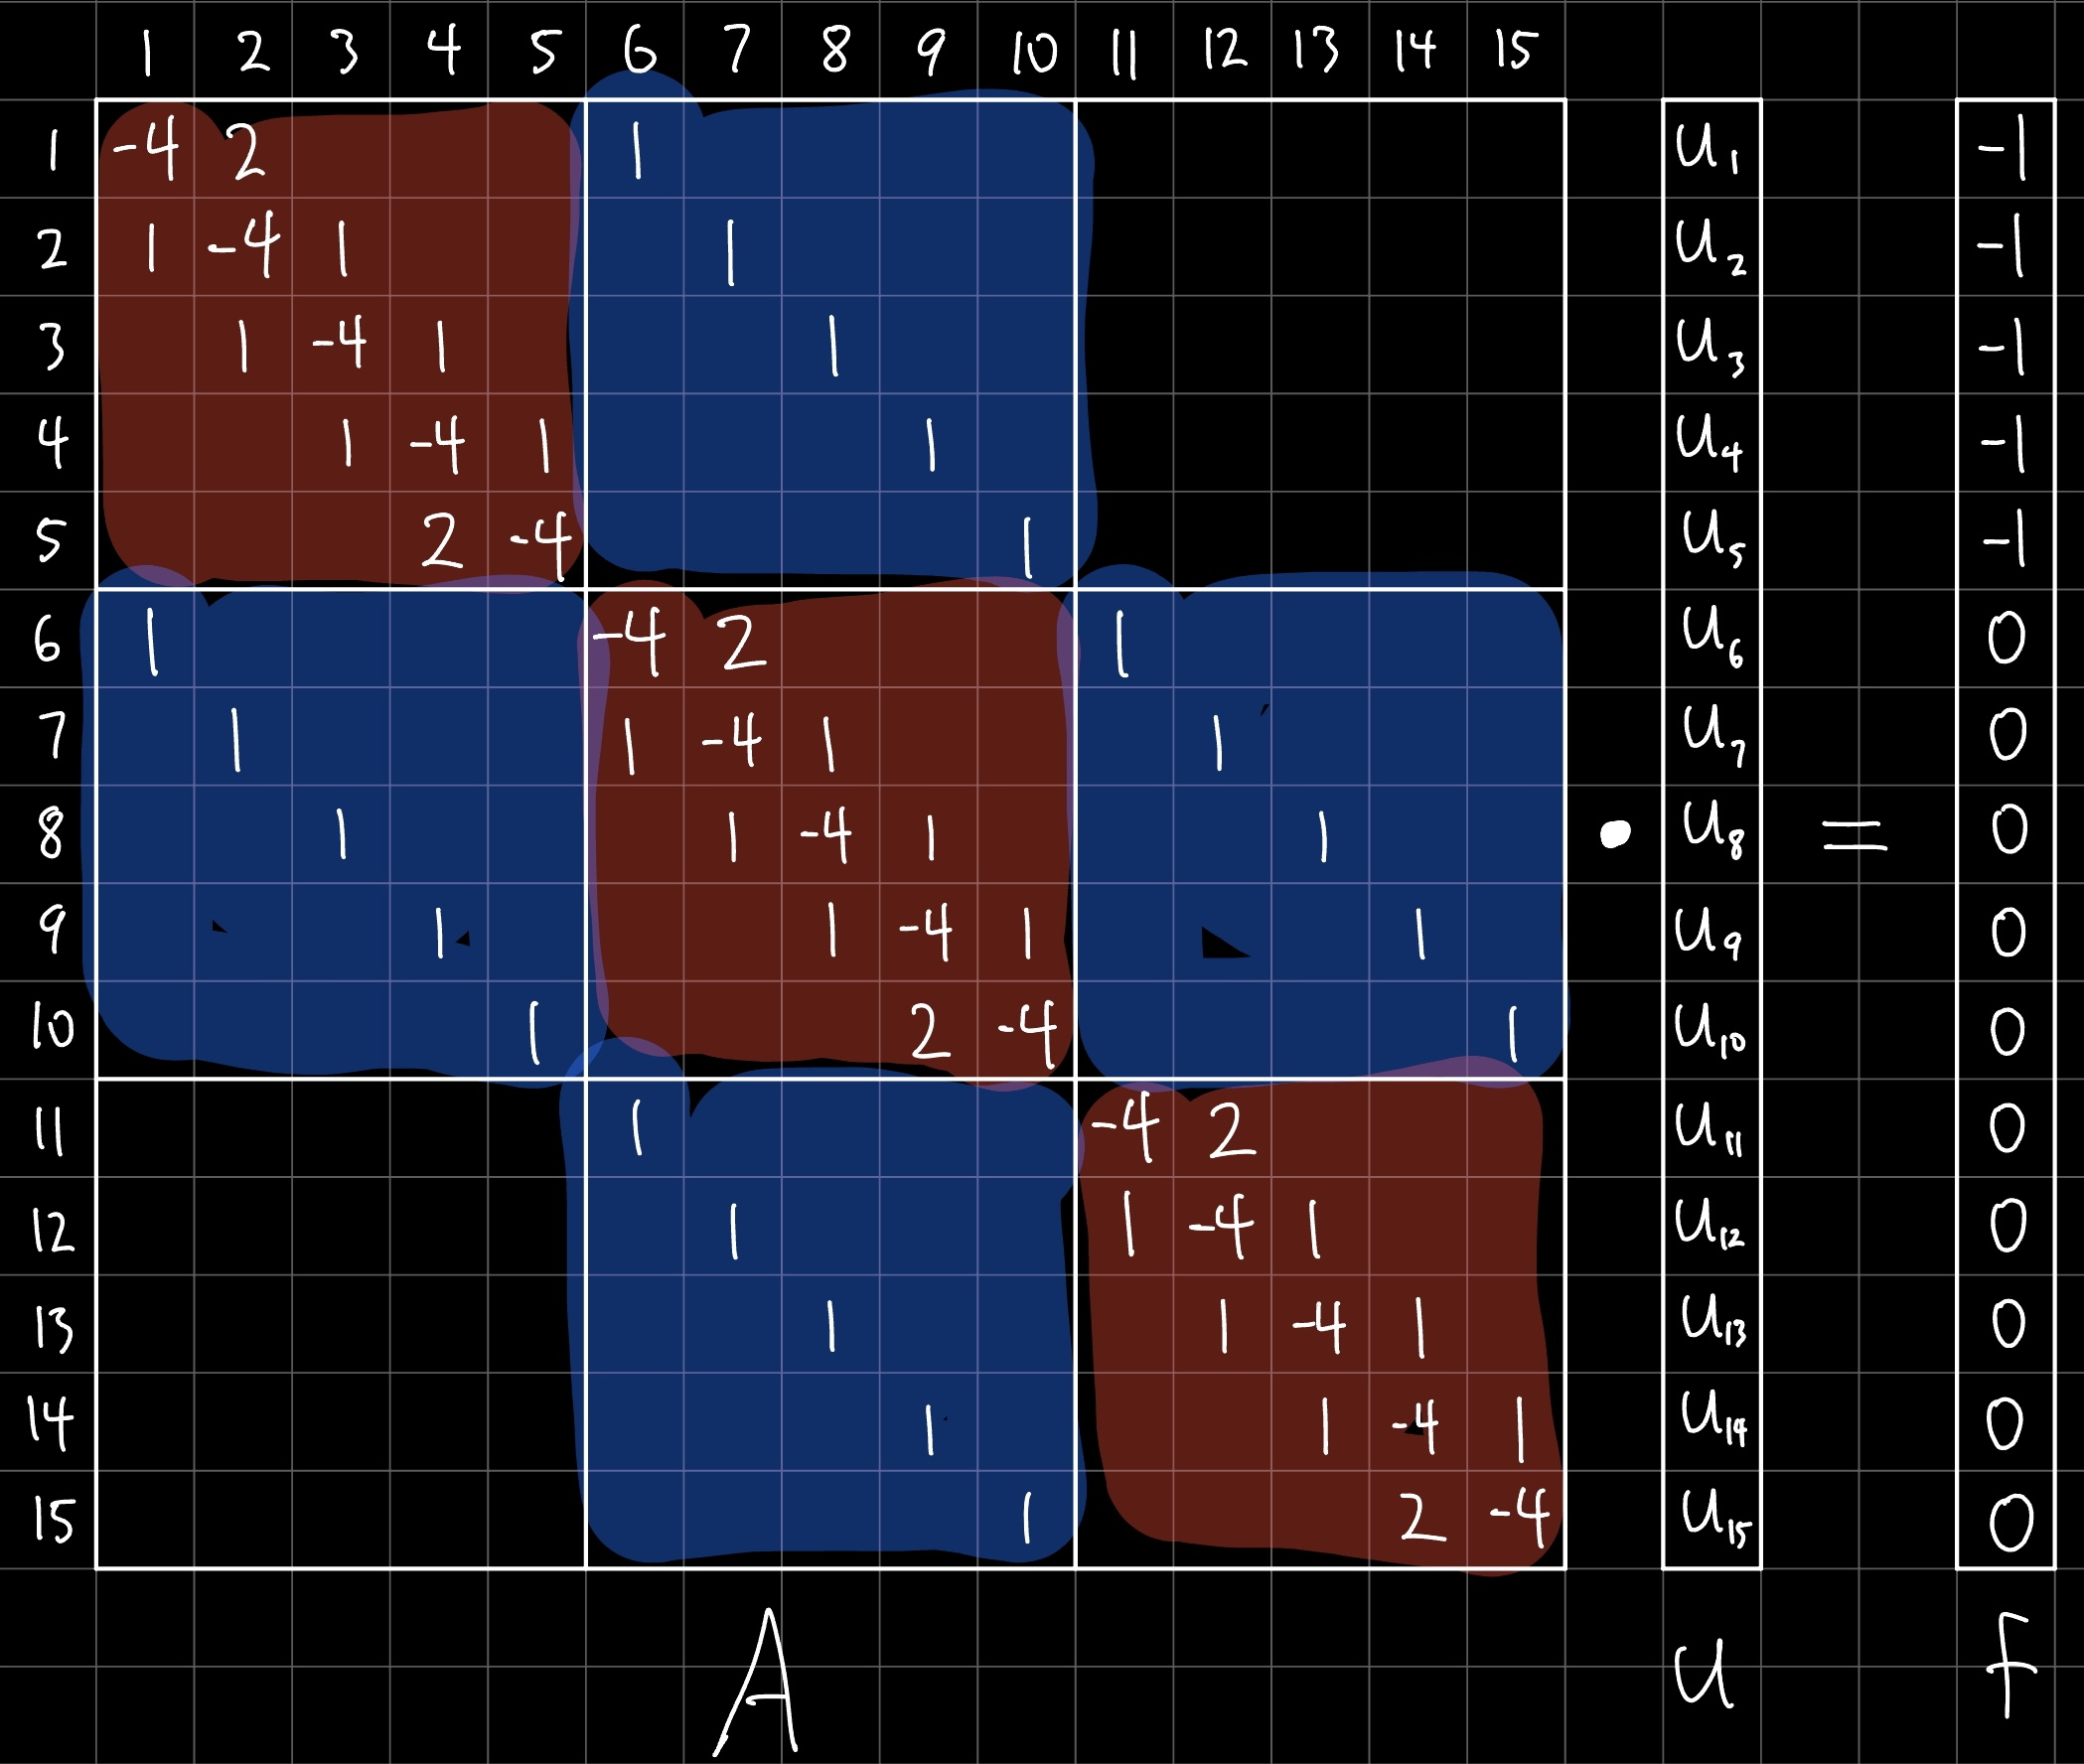
\includegraphics[scale=.1]{hw6 a full}
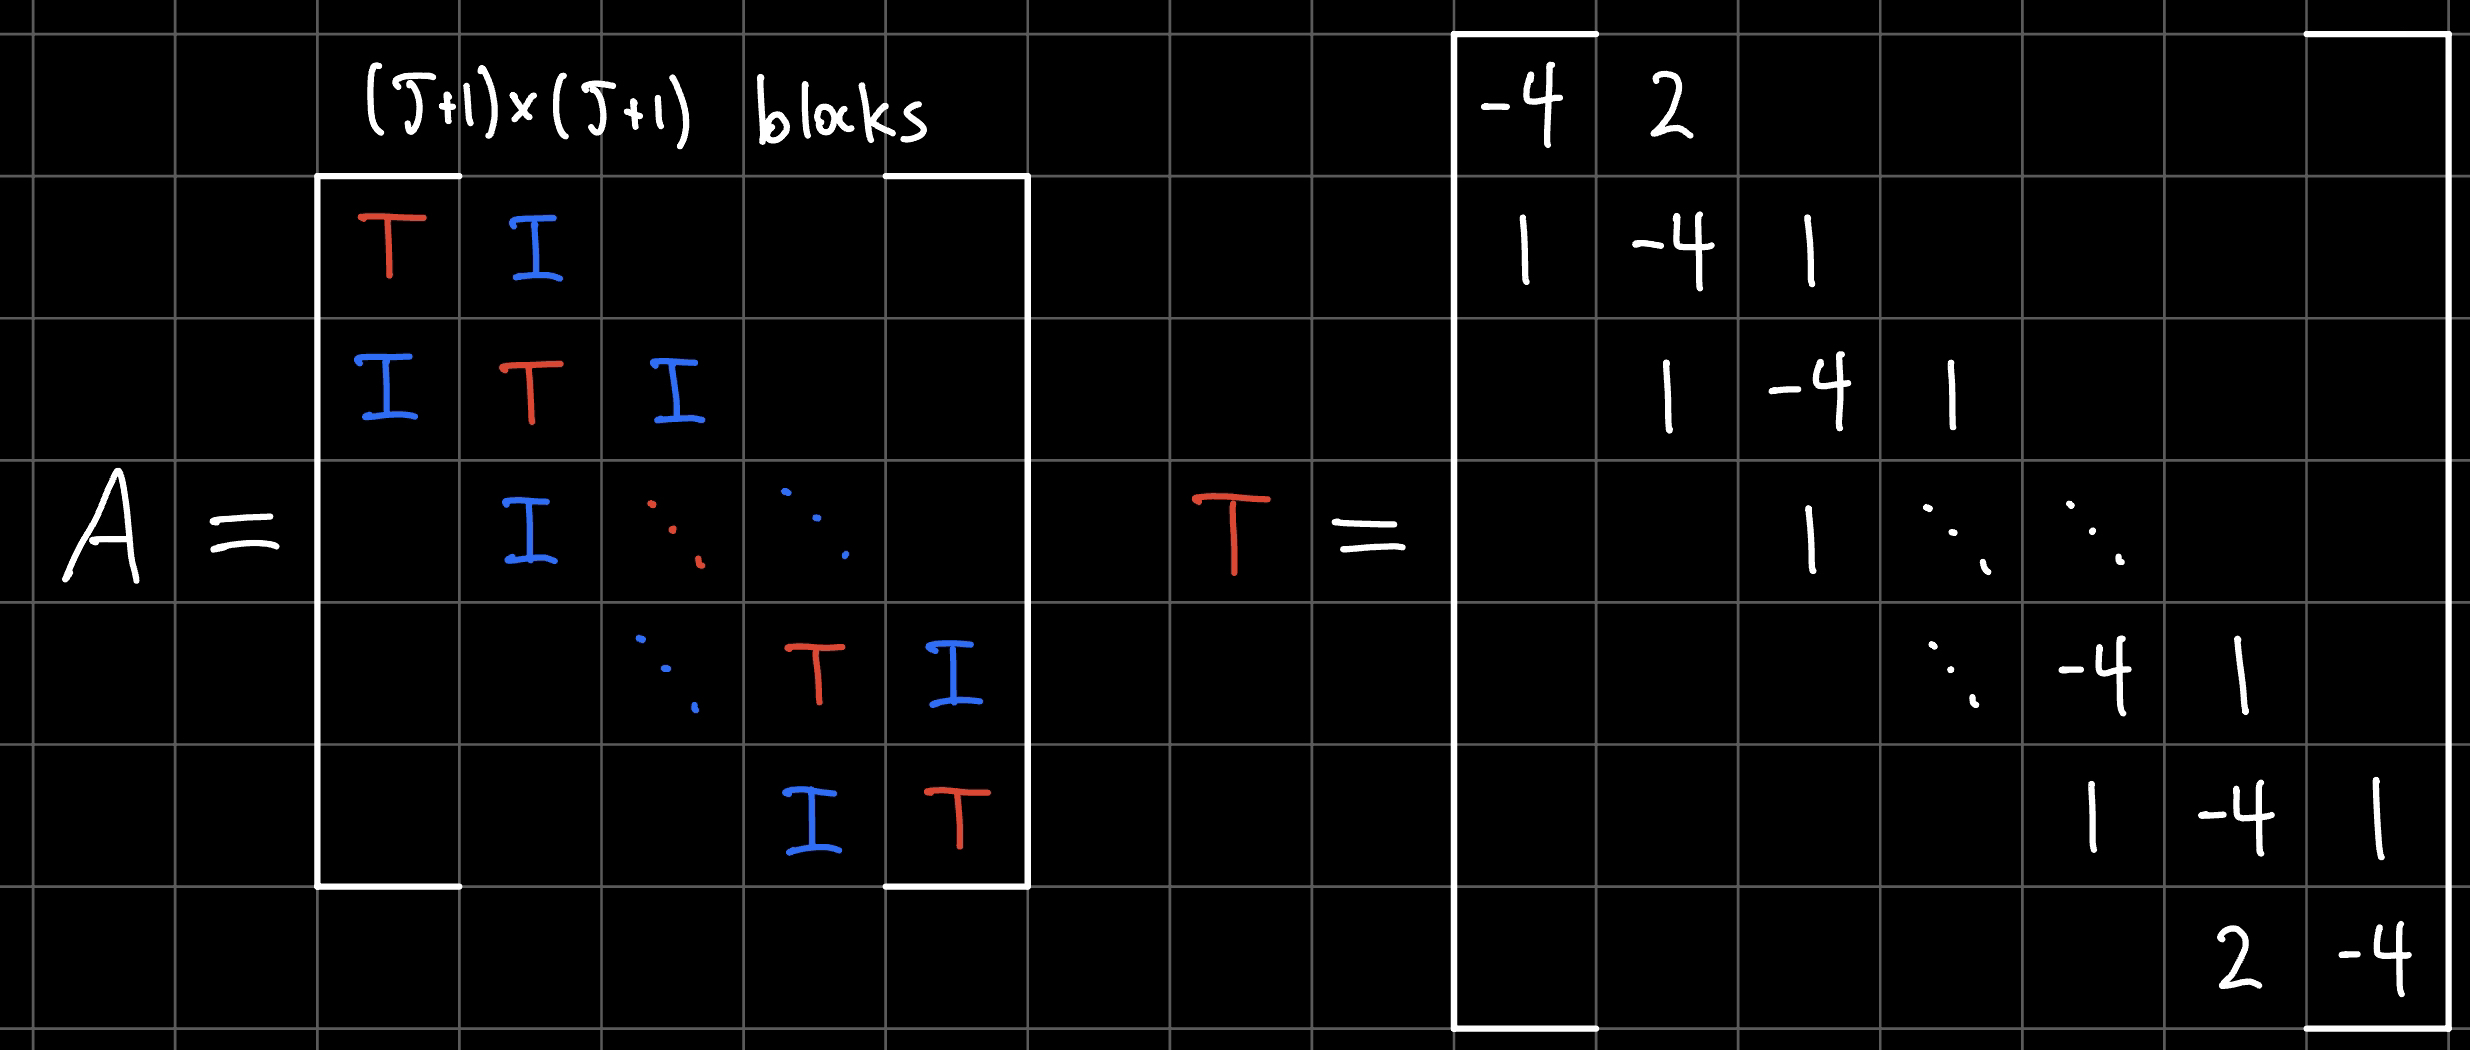
\includegraphics[scale=.09]{hw6 a block}


\item The system $Au=f$ is shown on the left, and the block structure of $A$ is compactly written on the right.

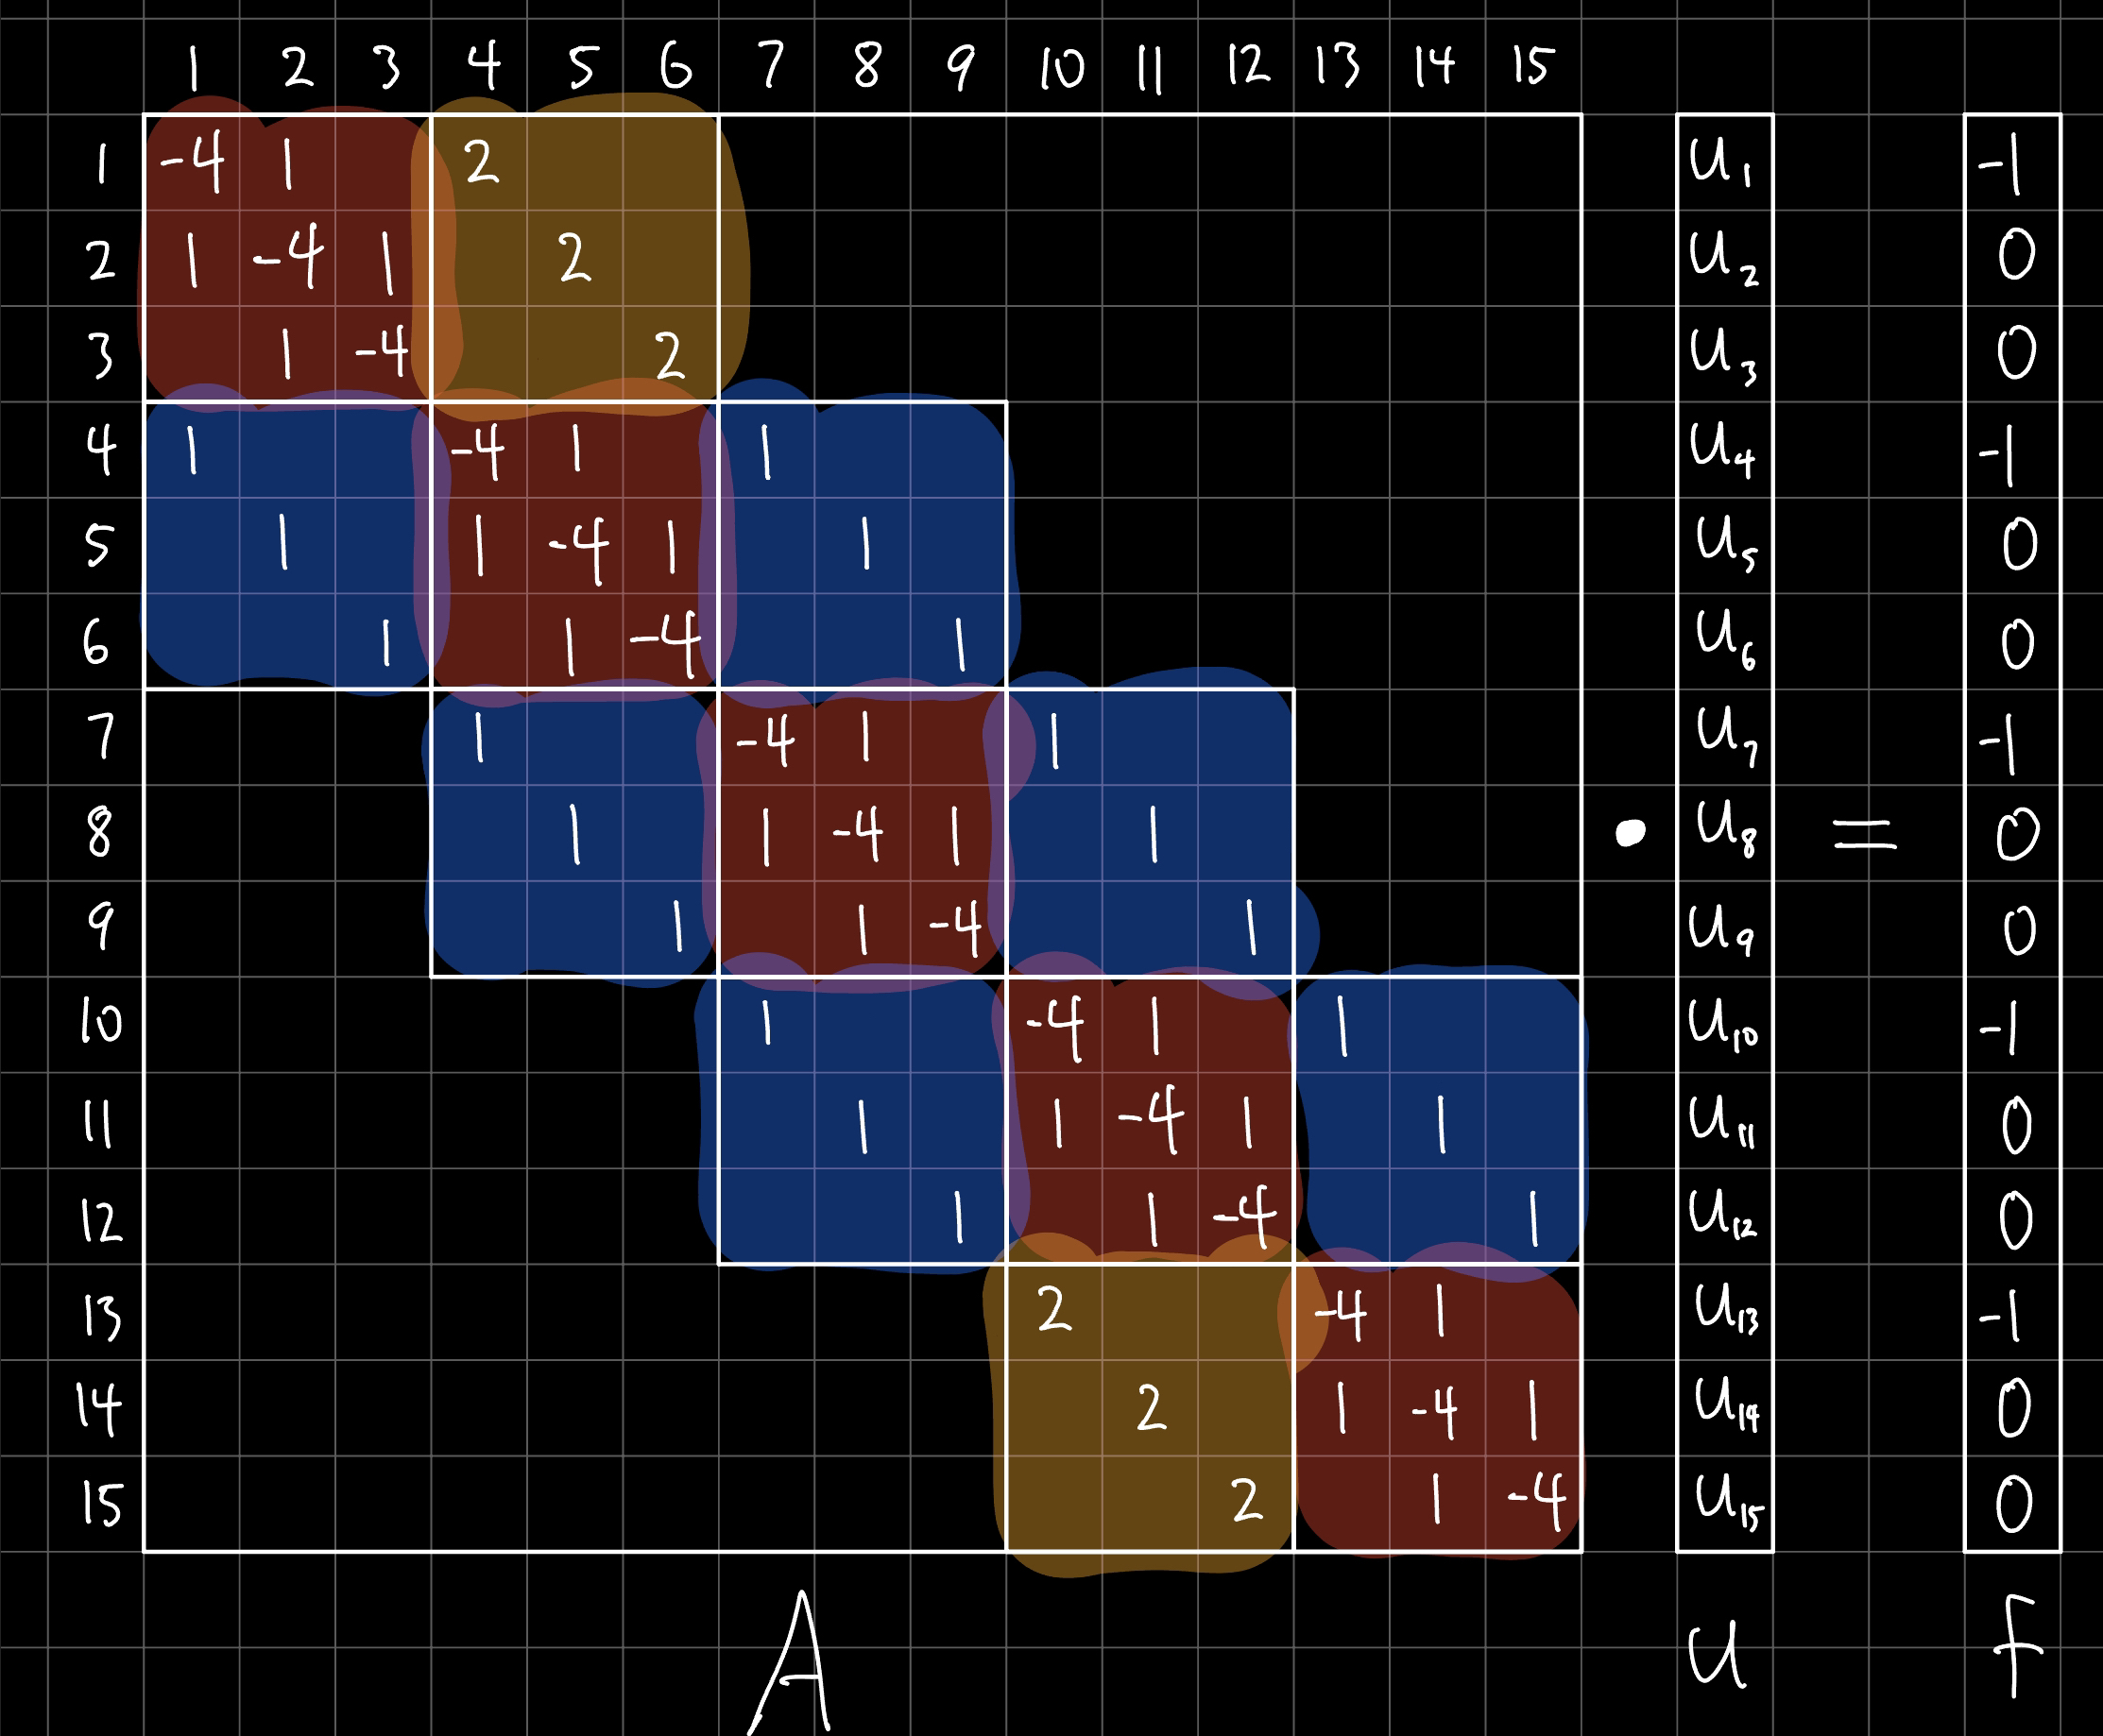
\includegraphics[scale=.1]{hw6 b full}
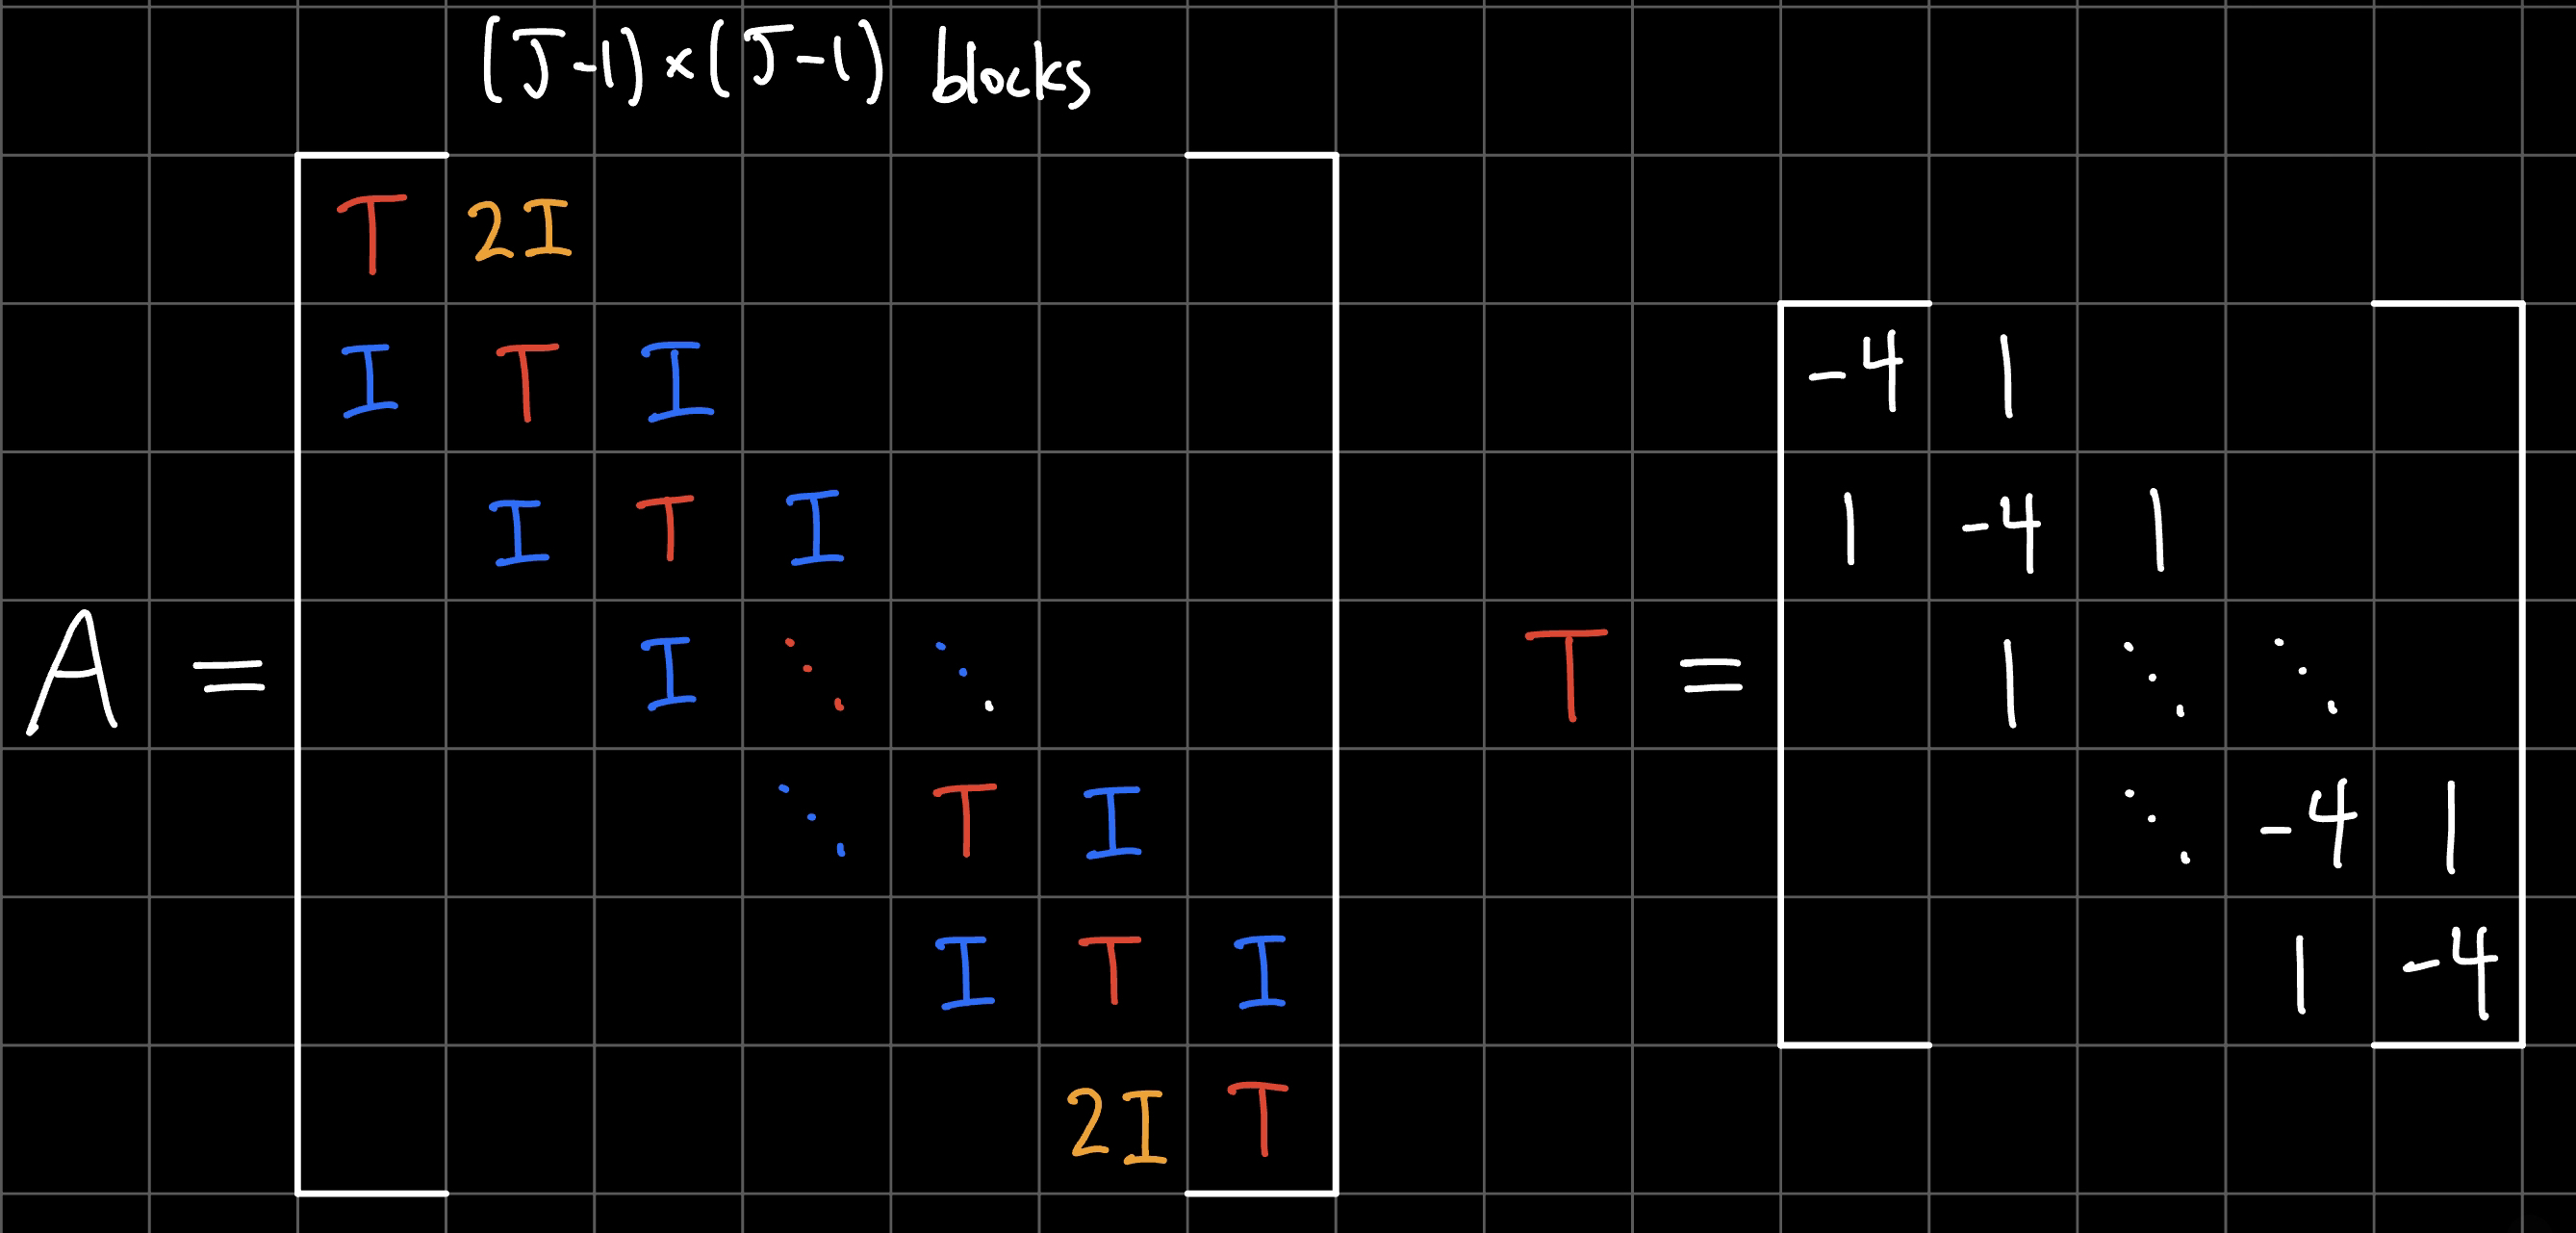
\includegraphics[scale=.08]{hw6 b block}


\item The system $Au=f$ is shown on the left, and the block structure of $A$ is compactly written on the right.

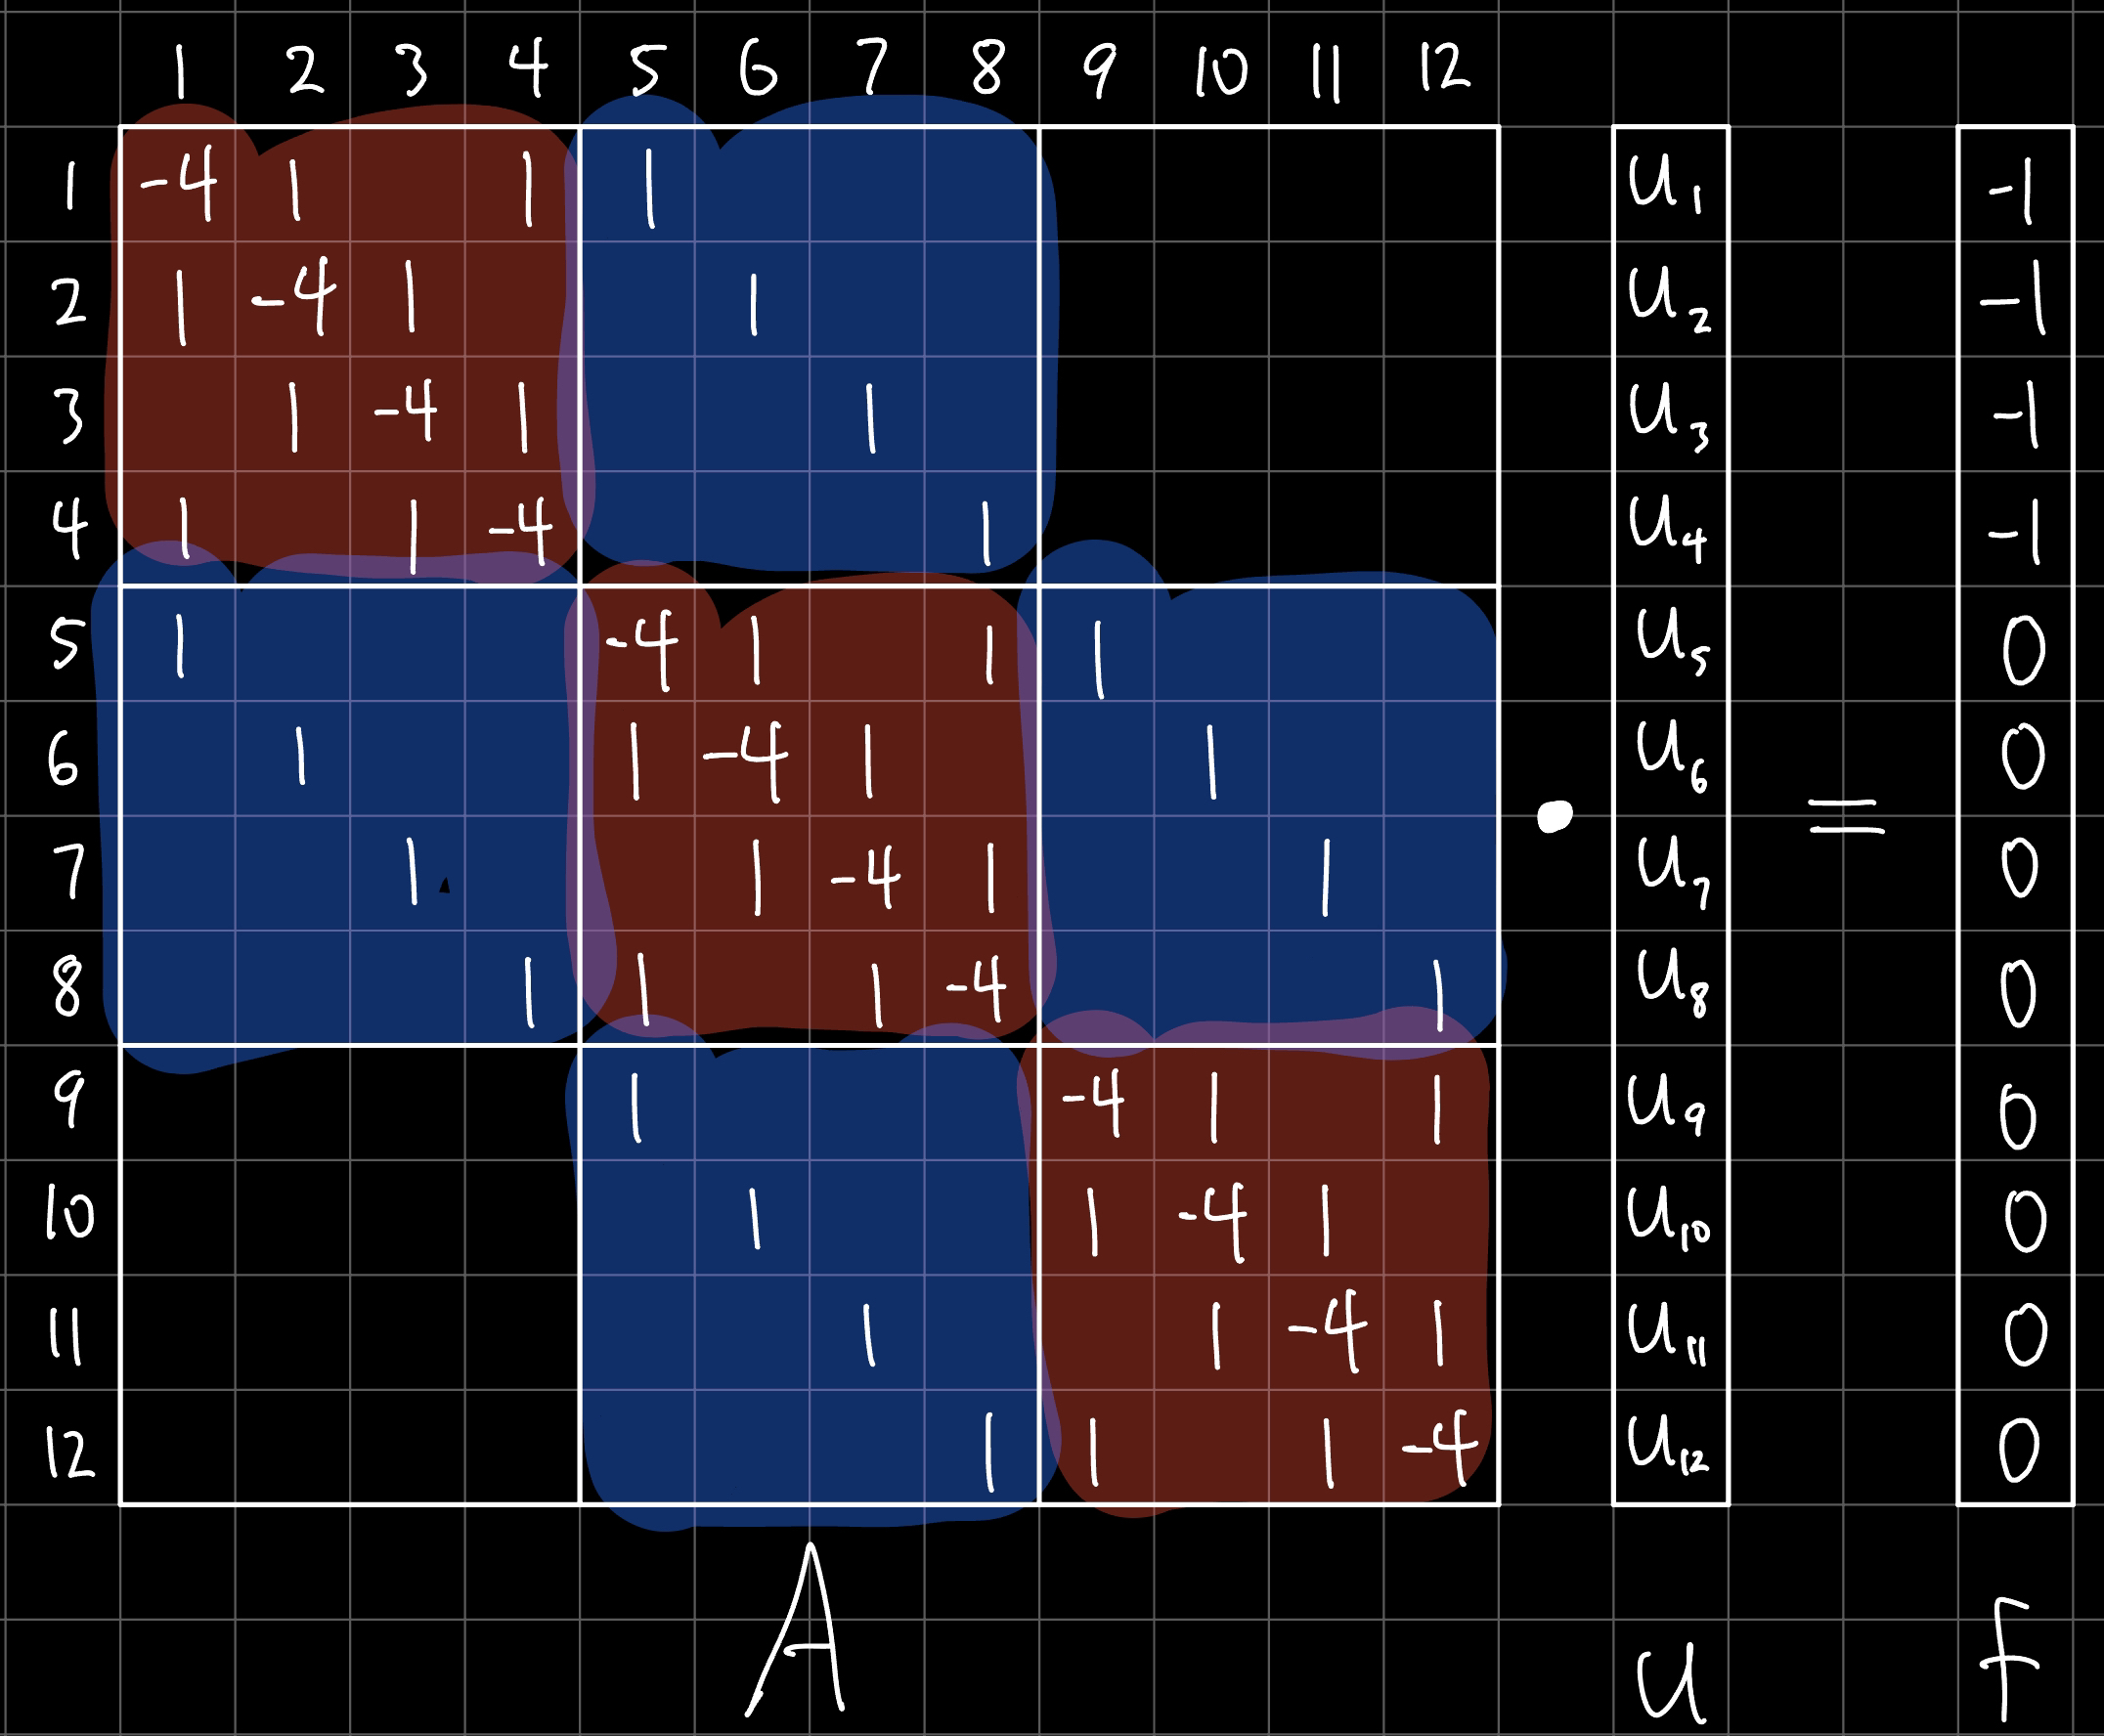
\includegraphics[scale=.1]{hw6 c full}
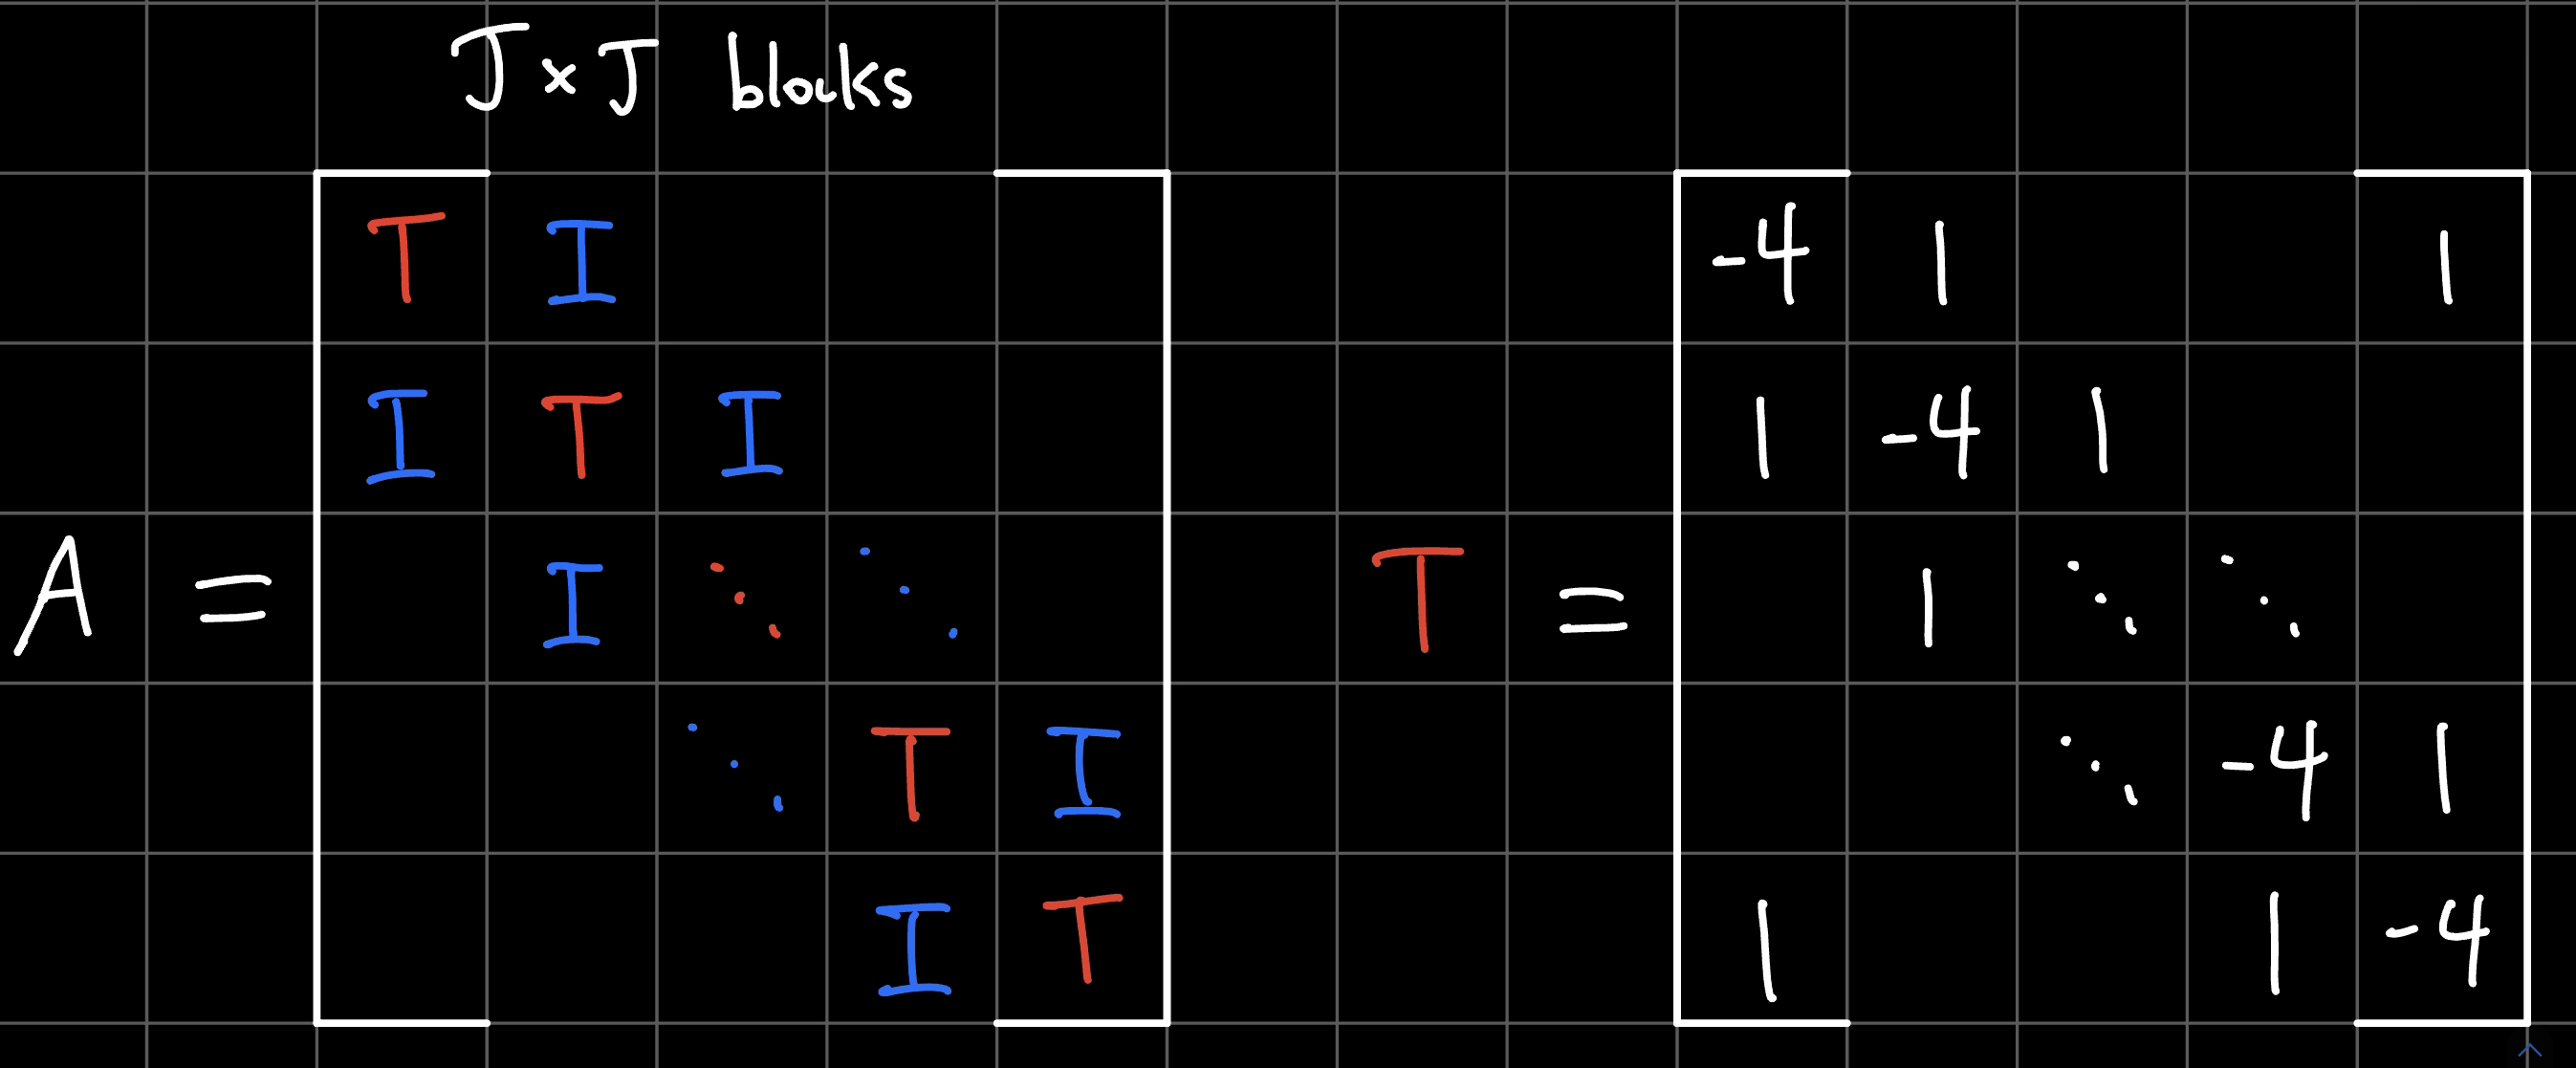
\includegraphics[scale=.08]{hw6 c block}


\item The system $Au=f$ is shown on the left, and the block structure of $A$ is compactly written on the right.

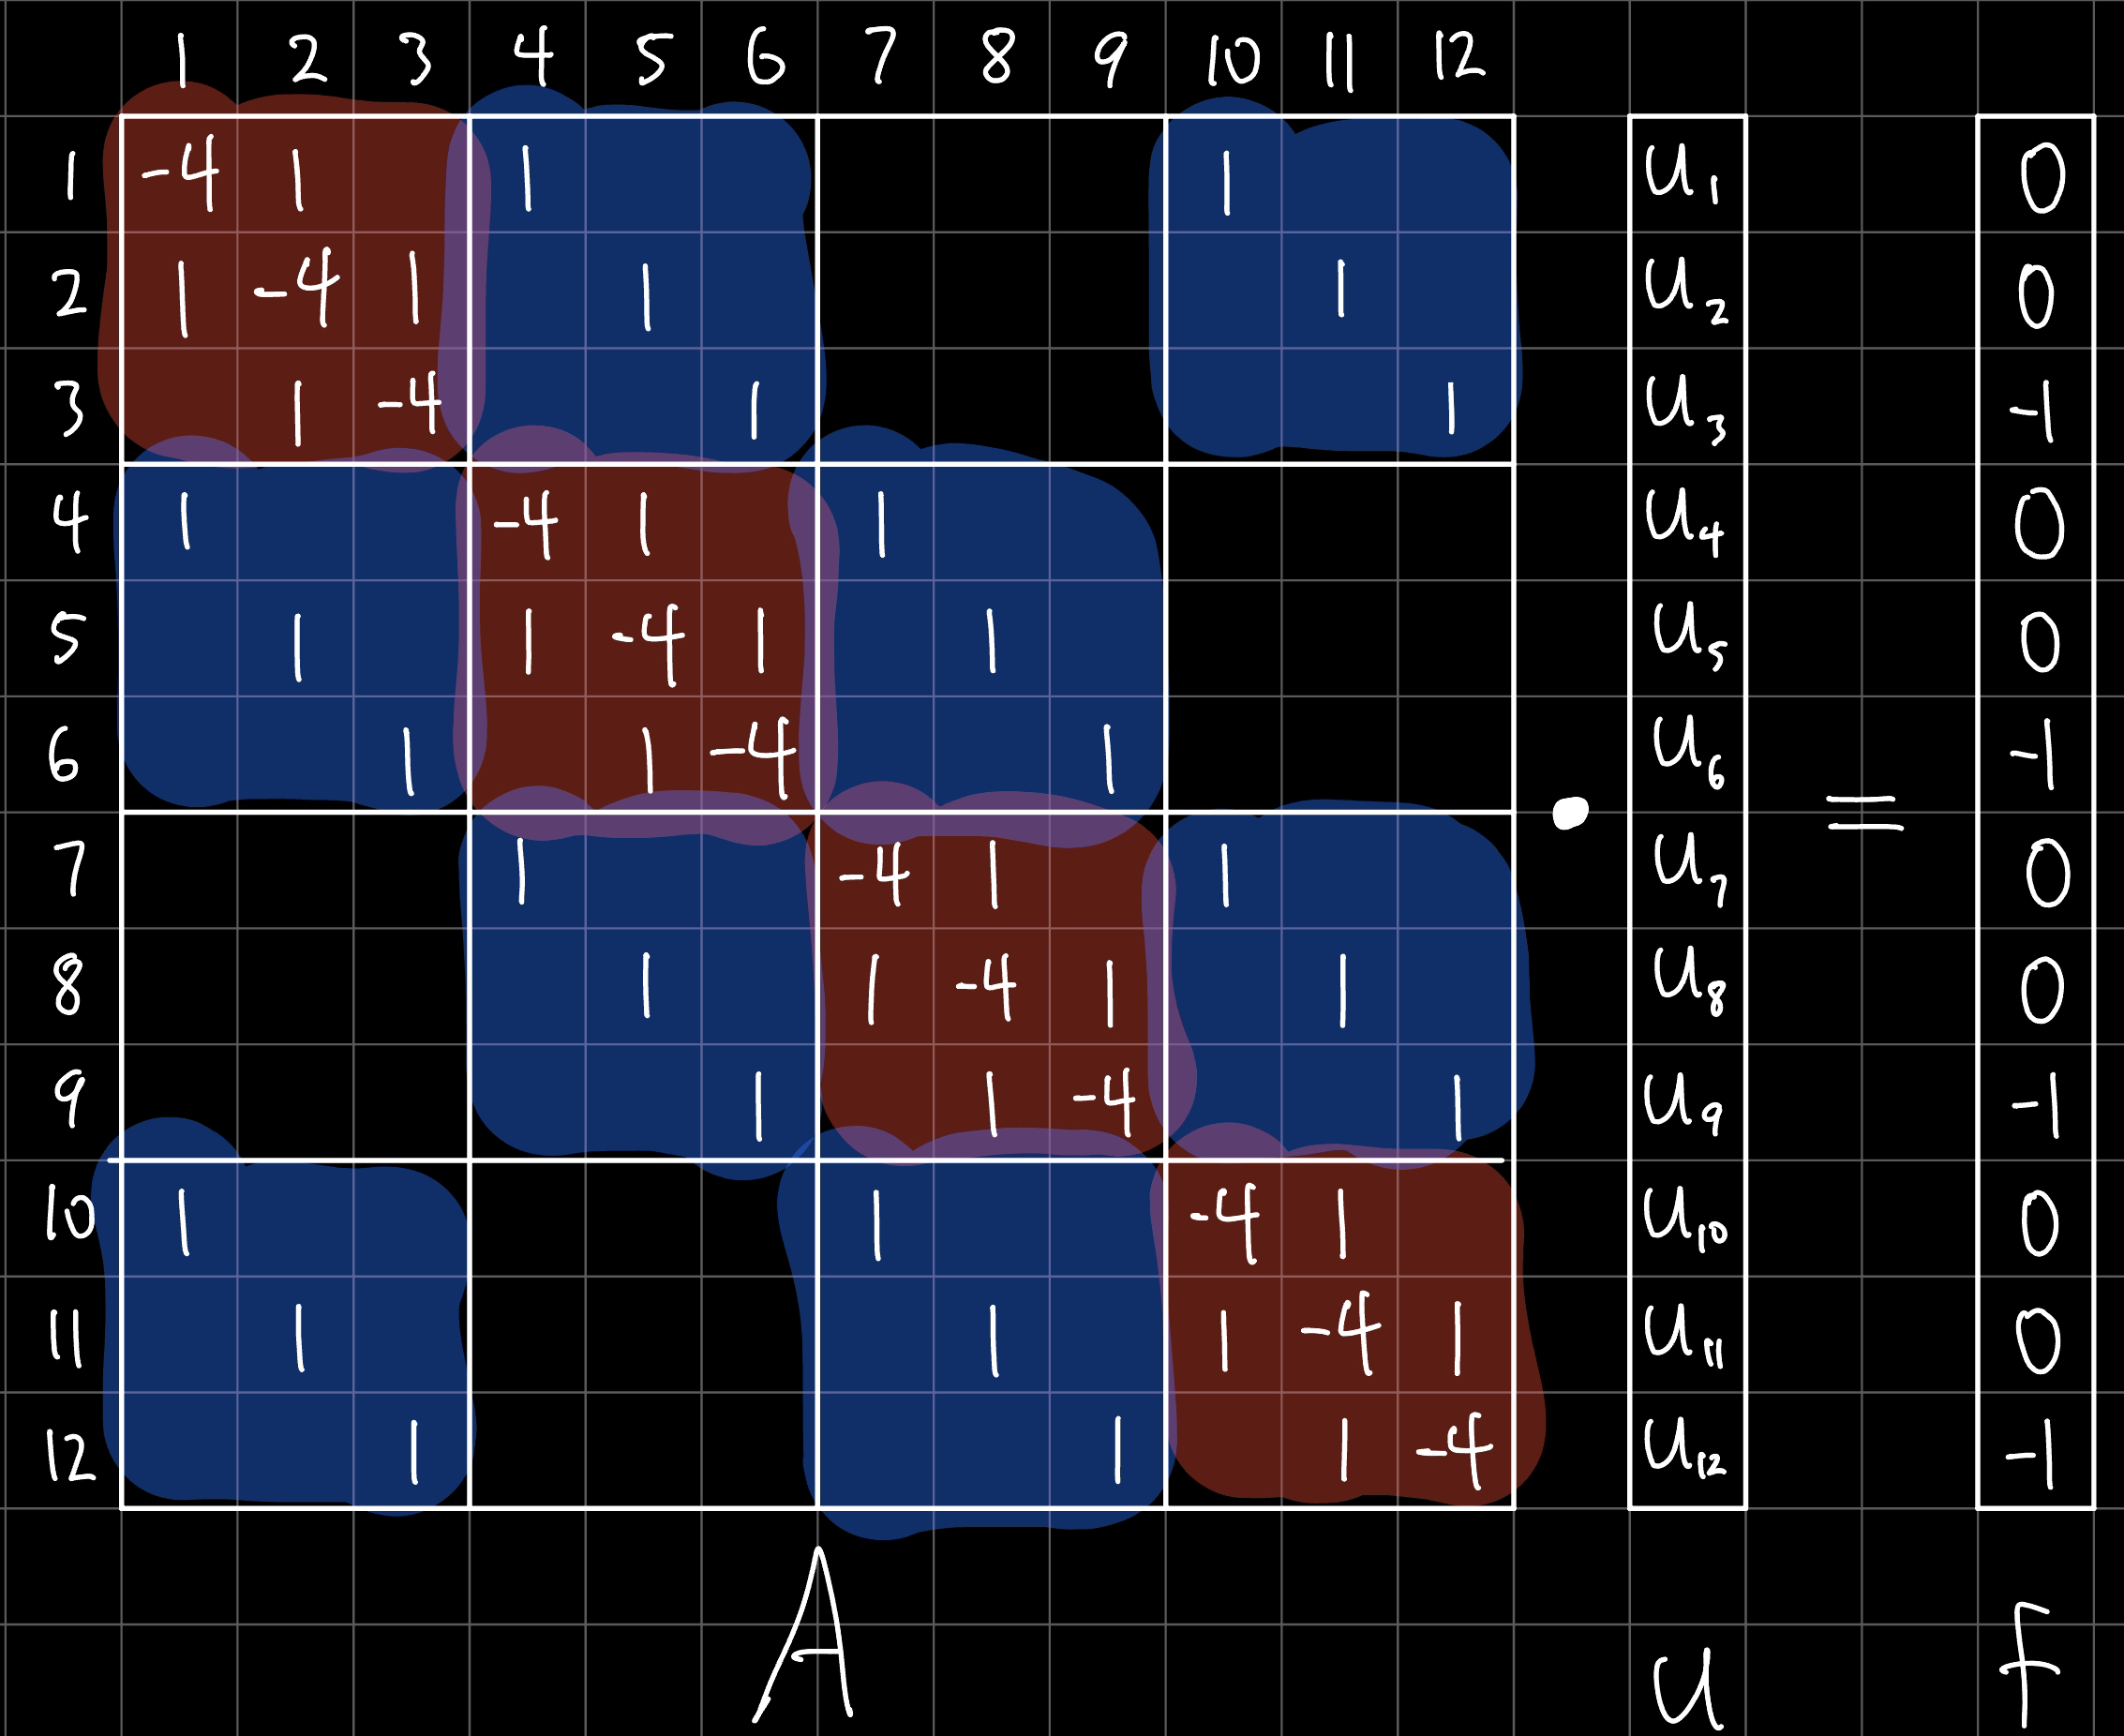
\includegraphics[scale=.1]{hw6 d full}
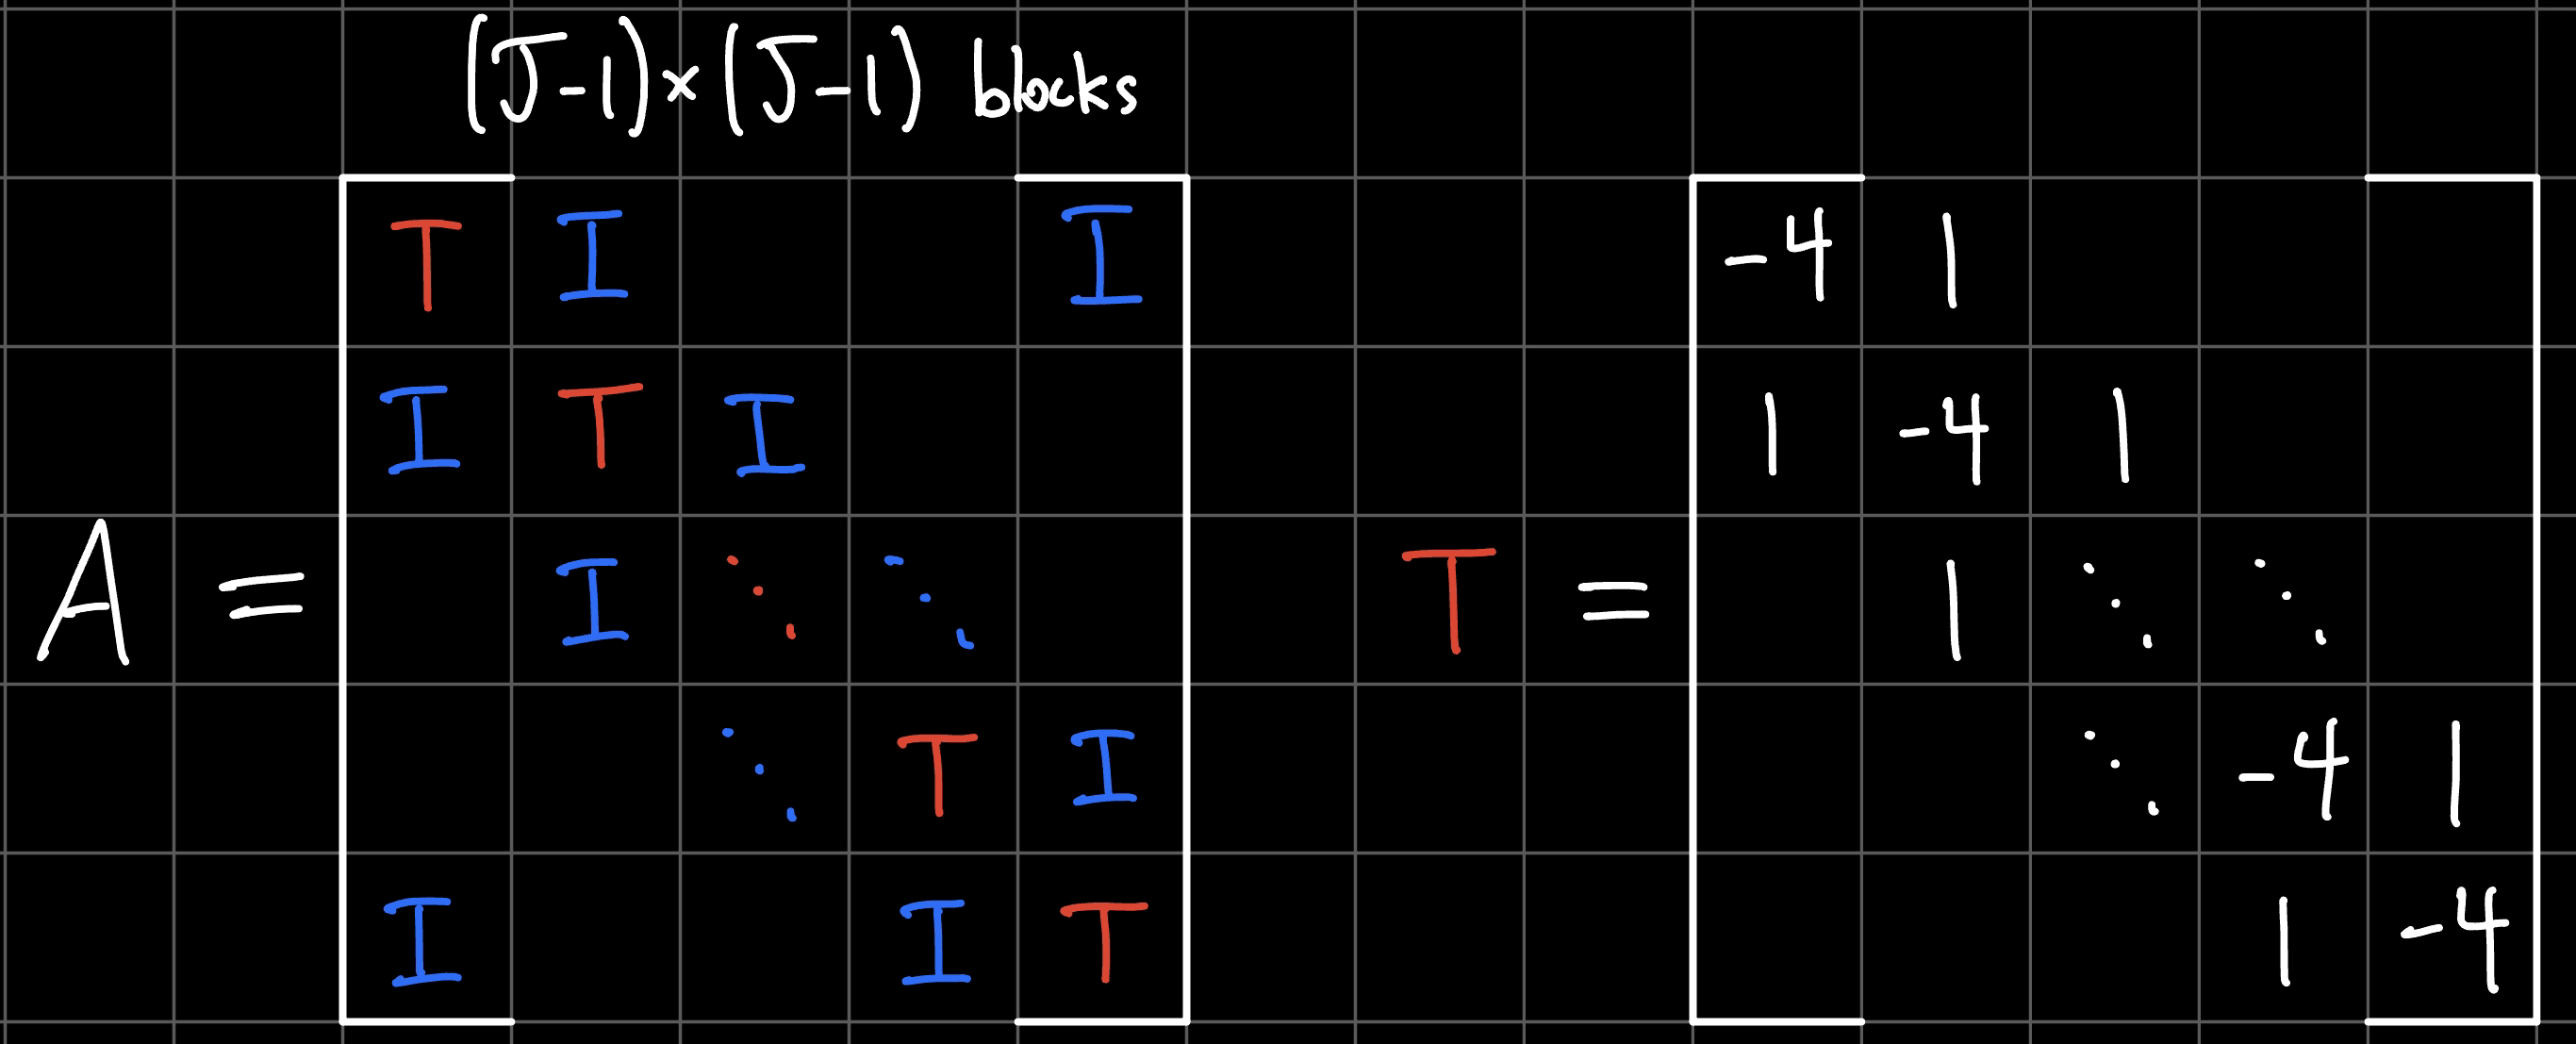
\includegraphics[scale=.08]{hw6 d block}


\item The system $Au=f$ is shown on the left. The block structure of $A$ is highlighted.

\begin{center}
	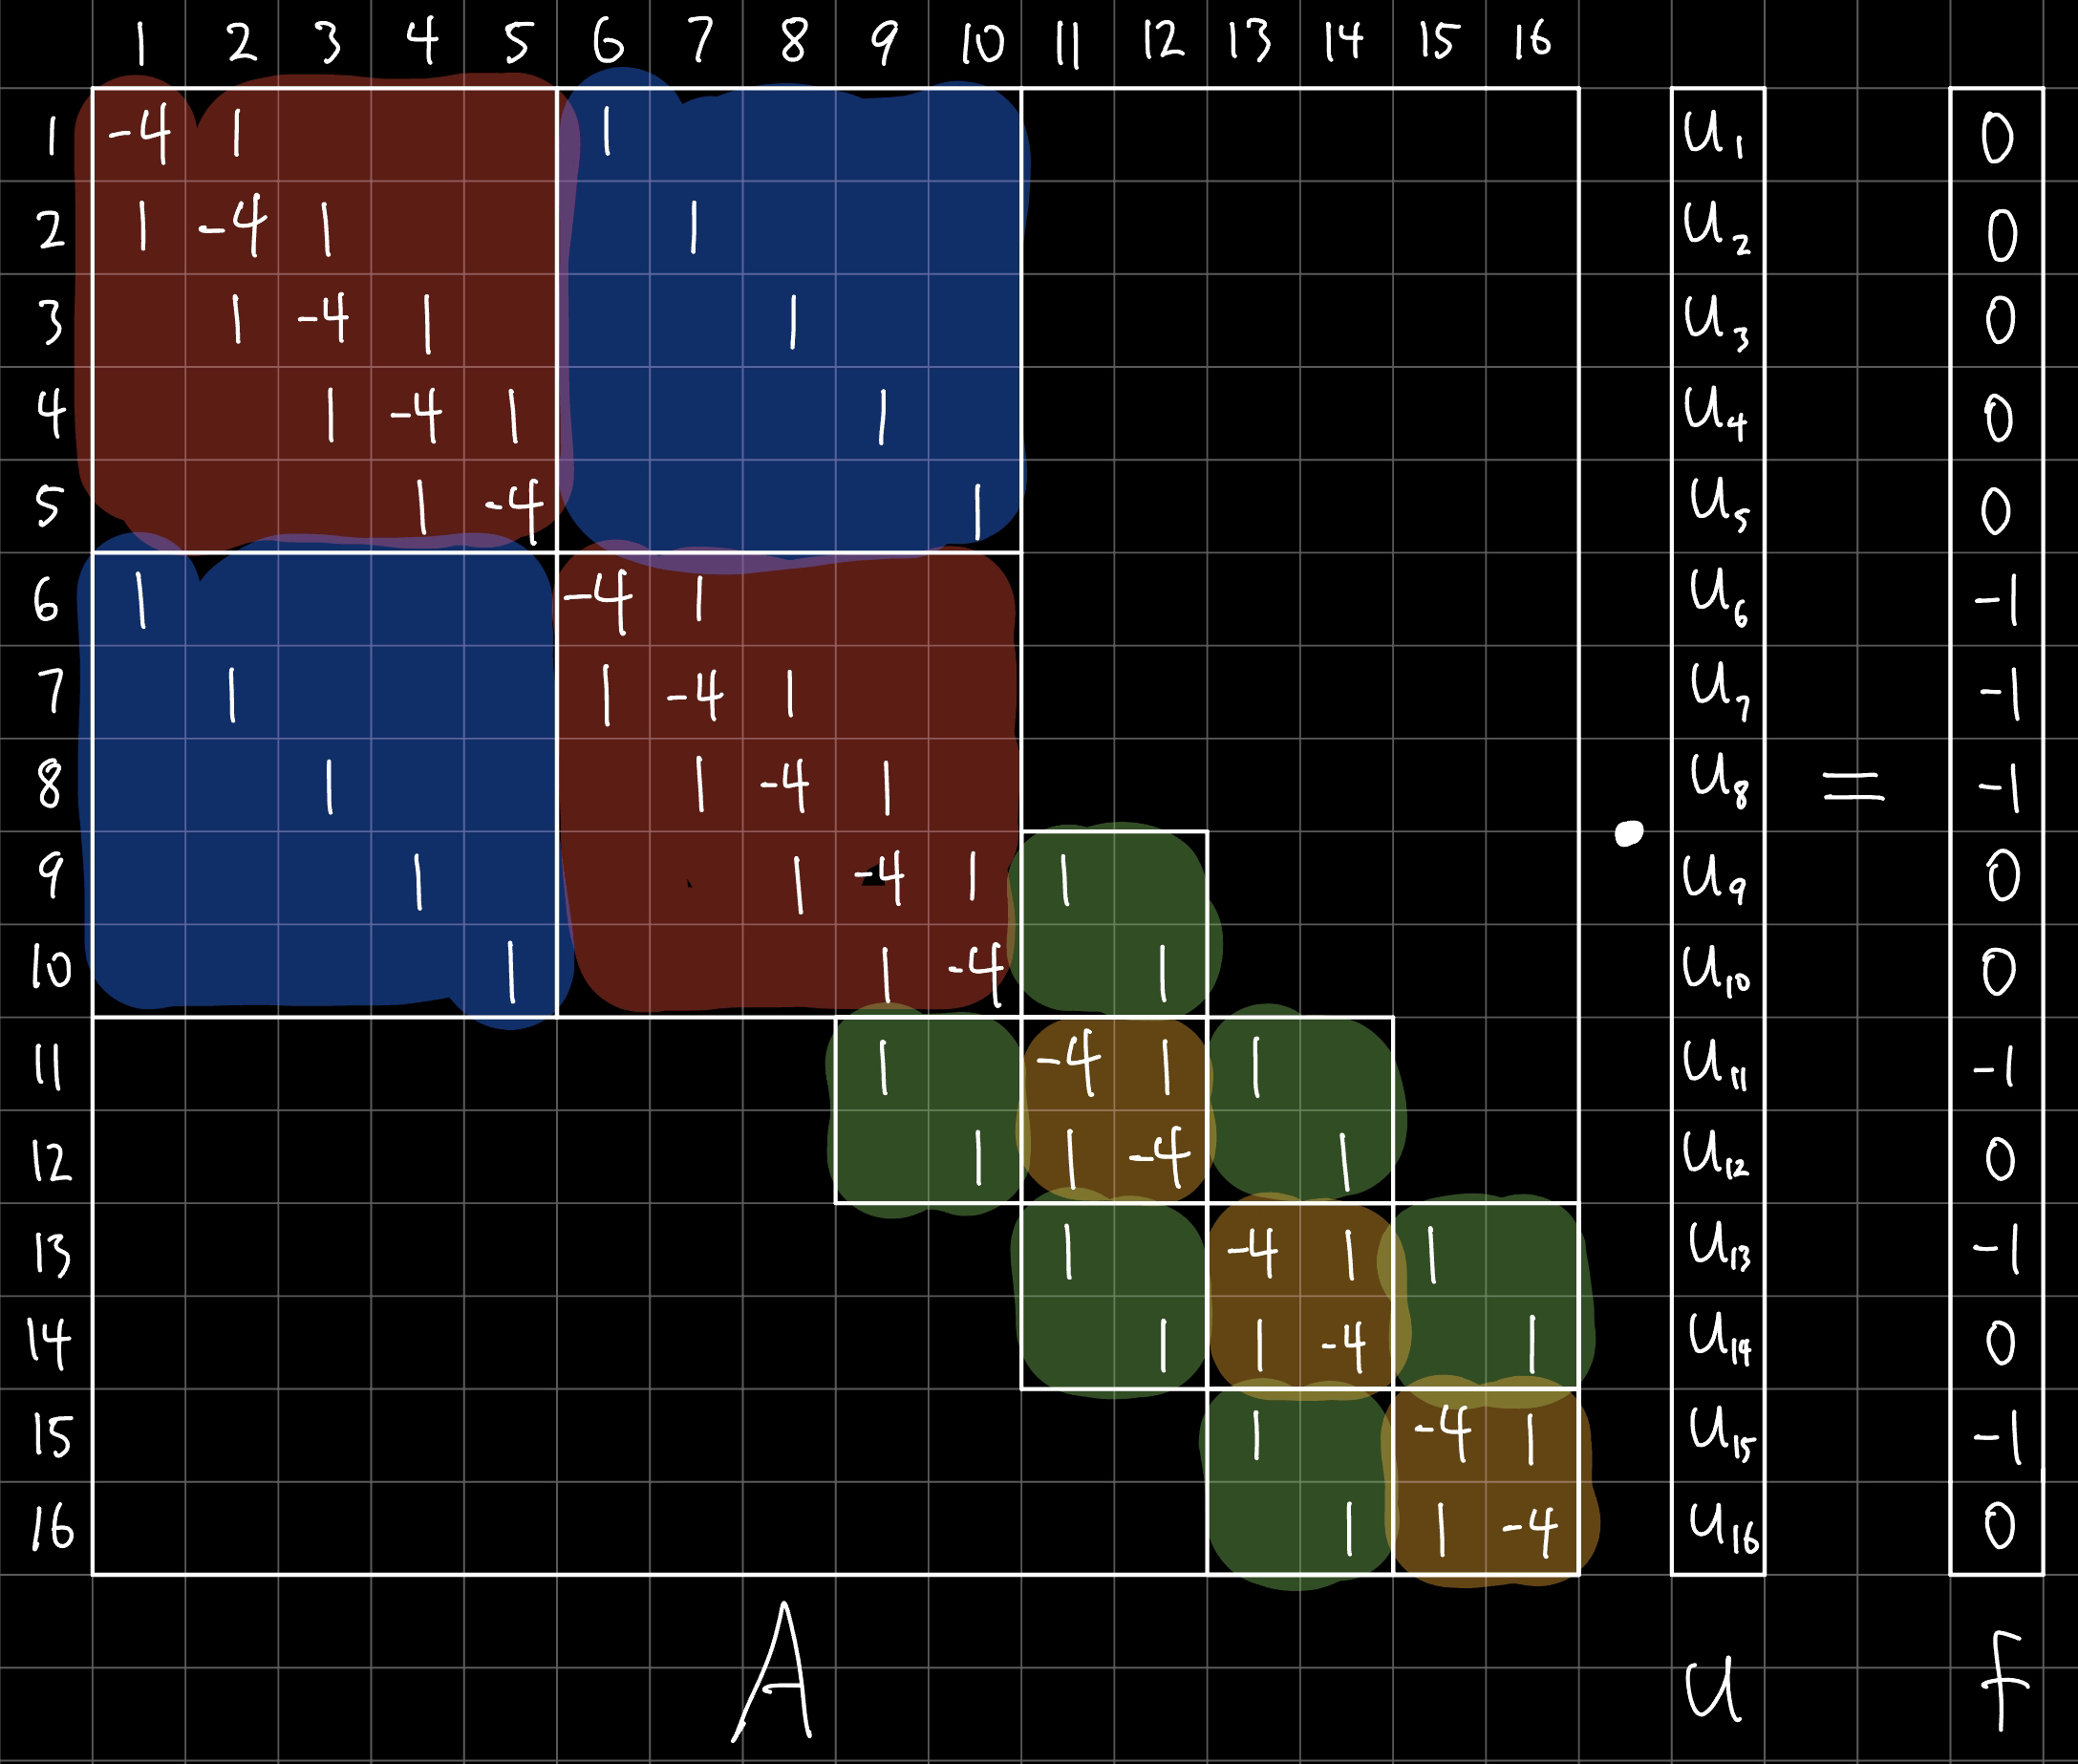
\includegraphics[scale=.1]{hw6 e full}
\end{center}
	
\end{enumerate}
\sep



\tbf{Problem 2.} The BVP on the domain $\Omega:=[-\pi,\pi]\times[0,2]$ is
$$u_{xx} + u_{yy} = g(x,y) :=
\begin{cases}
	-\cos x, & -\frac\pi2 \le x \le \frac\pi2\\
	0, & \text{else}
\end{cases}$$
with BCs
$$u\eval_{x=\pi} = u\eval_{x=-\pi},
\quad u_x\eval_{x=\pi} = u_x\eval_{x=-\pi},
\quad u\eval_{y=0} = 0,
\quad u_y\eval_{y=2} = 0$$

Fix $J\in\bN$. Set mesh steps in the $x$ and $y$ directions,
$$h_x := \frac{2\pi}{J},
\quad h_y := \frac{2}{J}$$
Then
$$u_{xx}(x,y) = \frac{1}{h_x^2}\sbr{u(x+h_x,y) - 2u(x,y) + u(x-h_x,y)} + O(h_x^2)$$
$$u_{yy}(x,y) = \frac{1}{h_y^2}\sbr{u(x,y+h_y) - 2u(x,y) + u(x,y-h_y)} + O(h_y^2)$$
Using the compass direction notation from lecture,
$$-2u_P\sbr{\frac{1}{h_x^2} + \frac{1}{h_y^2}} + \frac{1}{h_x^2}[u_E + u_W] + \frac{1}{h_y^2}[u_N + u_S] = g_P$$
Set $a:=\frac{1}{h_x^2},~b:=\frac{1}{h_y^2},~c:=a+b$, so that
$$-2cu_P + a[u_E + u_W] + b[u_N + u_S] = g_P$$

This creates a mesh from $\Omega$ with $(J+1)^2$ points. To explore the problem, take $J=4$. The corresponding mesh is shown below.

\begin{center}
	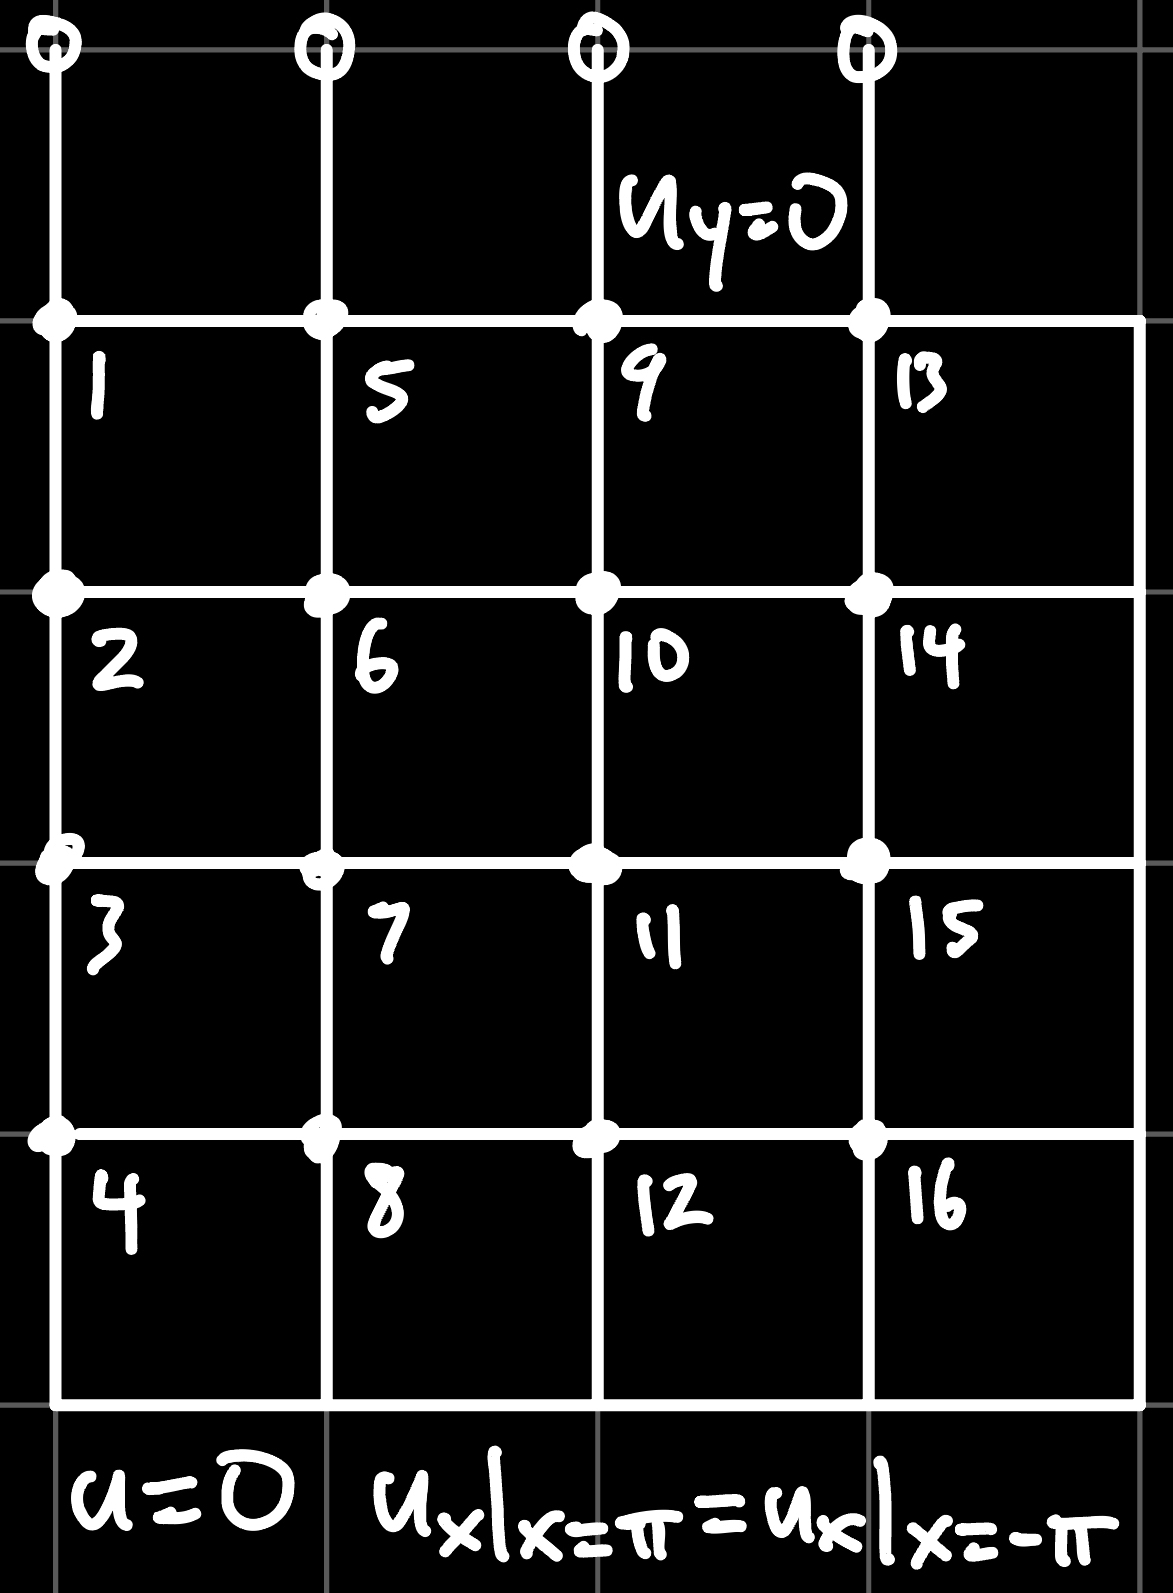
\includegraphics[scale=.1]{hw6 2 grid}
\end{center}

\end{document}